% Section content template for individual Educative lessons
% This file contains the actual content for a specific section
% Generated from Educative API section content

% Section: Sequence Diagram for ESPNcricinfo
% Section ID: 5017688209620992
% Section Slug: sequence-diagram-for-espncricinfo
% Generated: 2025-12-14T13:33:23.002357

Sequence diagrams are an effective way to visualize the interactions between different entities and objects within a system. There can be different sequence diagrams that we can create for the ESPNcricinfo system. In this lesson, we will create a sequence diagram for the following interaction:

\begin{itemize}
\item
\protect\phantomsection\label{WF7vd6yNUBS5xmkrskw8P}
\textbf{Add a match:~} The admin adds a new match to the system.
\end{itemize}

\subsection{Add a match}\label{m0UUdq9xswCxDBg-vK36V}
\\
The sequence diagram for adding a match should have the following actors and objects that will interact with each other:

\begin{itemize}
\item
\protect\phantomsection\label{zyN1vrztRaw9x1u75Paoz}
\textbf{Actors:} \texttt{Admin}, \texttt{Umpire}, and \texttt{Commentator}
\item
\protect\phantomsection\label{78zUBaoGyK9ksYjbV92lz}
\textbf{Objects:} \texttt{Match} and \texttt{Stadium}
\end{itemize}
\\
The steps involved in adding a match are listed below:

\begin{enumerate}
\item
\protect\phantomsection\label{_FGNct_vA6r-RuGSpcfQm}
The admin creates a new match of a specific match type.
\item
\protect\phantomsection\label{djCHdBTTvk00V70BD7Wgv}
The admin adds the playing teams for the match.
\item
\protect\phantomsection\label{-xSrjuVbPA9SsScfdvMCf}
The admin assigns a stadium to the match.
\item
\protect\phantomsection\label{ubXvTiJ-Y0w27qkPx2OeU}
The admin assigns an umpire to the match.
\item
\protect\phantomsection\label{duqWiU-Ag3ehkVCFnrKPk}
The admin assigns a commentator to the match.
\end{enumerate}
\\
Based on the order above, the sequence diagram for adding a match in the ESPNcricinfo system is provided below:

\begin{figure}[htbp]
 \centering
 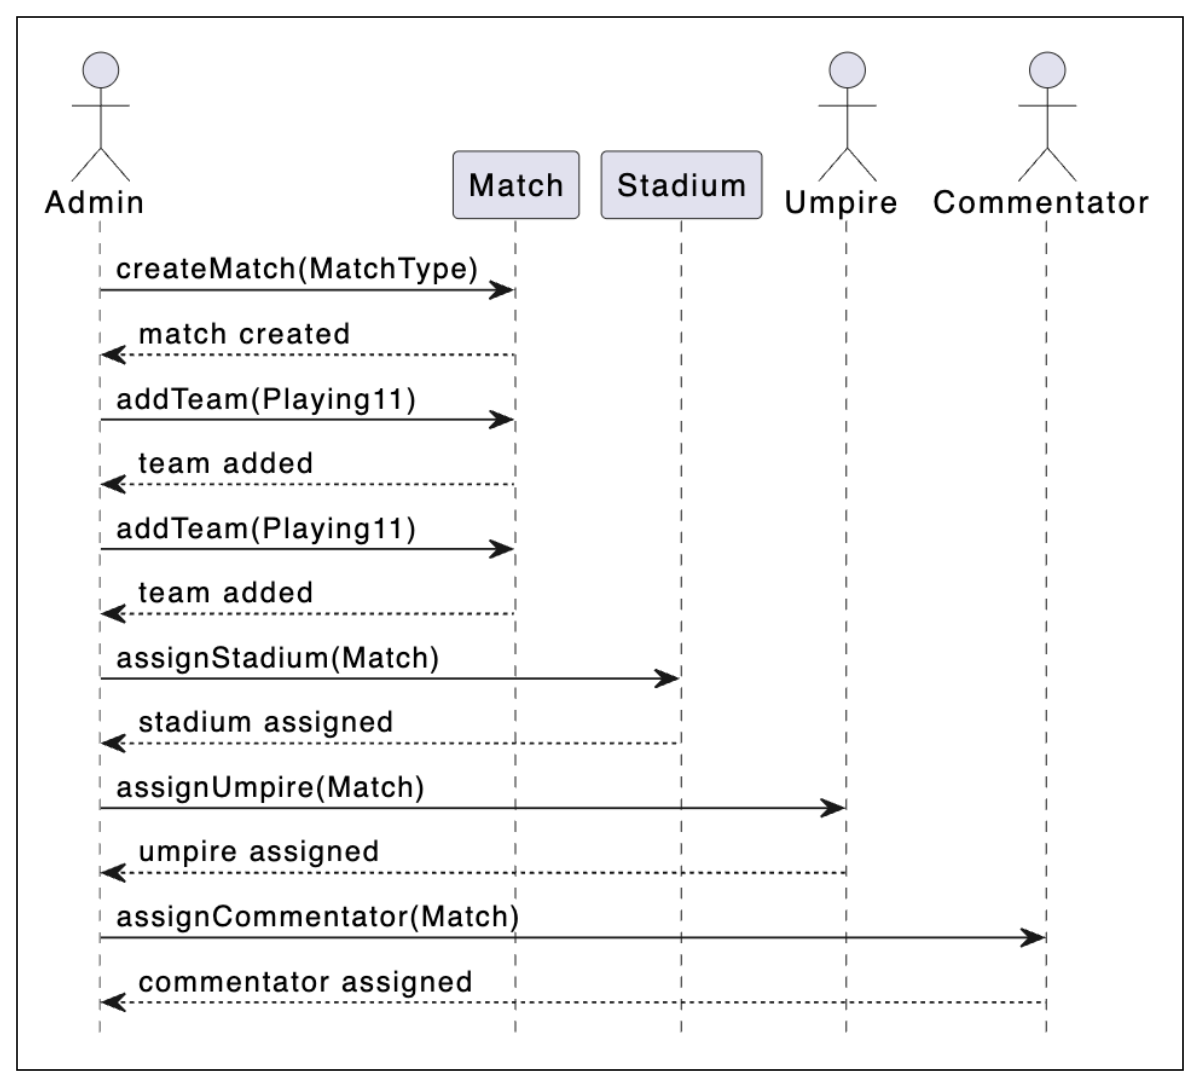
\includegraphics[width=0.5\textwidth]{Images/chapter_26/section_5017688209620992/5465986160263168.png}
 \caption{The sequence diagram for adding a match}
\end{figure}

Next, let's look at the activity diagrams for ESPNcricinfo to understand the system's control flow.

% End of section content